\documentclass[a4paper]{jsarticle}
\usepackage[dvipdfmx]{graphicx}
\usepackage[all]{xy}
\usepackage{../math_note, exercise}
\renewcommand{\thesection}{Ex2.\arabic{section}}

\newcommand{\shO}{\mathcal{O}}
\newcommand{\Sch}{\mathbf{Sch}}
\newcommand{\Var}{\mathbf{Var}}
\newcommand{\Rings}{\mathbf{Rings}}
\newcommand{\red}[1]{#1_{\text{red}}}
\newcommand{\basesp}{\operatorname{sp}}
\newcommand{\CoverU}{\mathfrak{U}}
\newcommand{\OpenIn}{\text{ :: open in }}
\newcommand{\ClosedIn}{\text{ :: open in }}

\begin{document}

\section{$(D(f), \shO_X|_{D(f)}) \homeo (\Spec A_f, \shO_{\Spec A_f})$} %% Ex2.1 
    $A$ :: ring, $X=\Spec A$, $f \in A$とし,$D(f)=(V((f)))^c$とする.
    $S=\{1,f,f^2,\dots\}$とし,以下のように写像を定める.
    \begin{defmap}
        \phi:& D(f)& \to& \Spec A_f \\ 
        {}& \I{p}& \mapsto& S^{-1}\I{p} \\
        {}& \I{q} \cap A& \mapedfrom& \I{q}
    \end{defmap}
    $\I{p}$は$S$と共通部分を持たない素イデアルだから,
    Ati-Mac Prop3.11より,$\phi$は全単射.

    $C \ClosedIn D(f)$とする.
    この時,
    \[ C=\{ \I{p} \in \Spec A ~|~ \I{I} \subseteq \I{p}, (f) \not \subseteq \I{p} \} \]
    となるイデアル$\I{I} \subset A$が存在する.
    Ati-Mac Prop3.3より,$\phi$は単射を保つから,$\phi(C)$もclosed.
    逆に$D \ClosedIn \Spec A_f$をとる.
    再びAti-Mac Prop3.11より,$\Spec A_f$の任意の元は拡大イデアルだから,
    \[ D=\{ \phi(\I{p}') \in \Spec A_f ~|~ \phi(\I{I}') \subseteq \phi(\I{p}'), \phi(f) \not \subseteq \phi(\I{p}') \} \]
    と書ける.
    つまり,$D=\phi(V(\I{I'}))$.
    $\phi$は全単射なので$\phi^{-1}(D)=V(\I{I'})$となり,これはclosed.
    以上より$\phi$が同相写像であることがわかった.

    Prop2.3と同様にlocally ringed spaceの射を構成しておく.
    これは
    \[ f: \I{p} \mapsto \phi^{-1}(\I{p}),~~ f^{\#}: \shO_{\Spec A_f}(-) \mapsto \shO_X|_{D(f)}(\phi(-)) \]
    で定義される.

\section{IF $X$ :: scheme, and $U \OpenIn X$, then $(U,\shO_X|_U)$ :: scheme.} %% Ex2.2 
    $X$はschemeだから,開被覆$\{U_{\lambda}\}_{\lambda \in \Lambda}$が存在し,
    $(U_{\lambda}, \shO_X|_{U_{\lambda}})$はaffine schemeとなる.
    すなわち,
    $R_{\lambda}$ :: ringが存在して
    \[ (U_{\lambda}, \shO_X|_{U_{\lambda}}) \homeo (\Spec R_{\lambda}, \shO_{\Spec R_{\lambda}}) \]
    と書ける.

    $V_{\lambda}=U \cap U_{\lambda}$とすると,$\{V_{\lambda}\}$は$U$の開被覆である.
    そして各$V_{\lambda} \subseteq U_{\lambda}$はaffine schemeの開集合.
    教科書pp.70-71から,affine schemeのopen baseは
    $D(f)~(f \in R_{\lambda})$の形の開集合全体である.
    したがって,各$V_{\lambda}$について,
    以下のような条件を満たす$R_{\lambda}$の部分集合$F_{\lambda}$が取れる.
    \[ V_{\lambda}=\bigcup_{f \in F_{\lambda}} D(f). \]
    まとめると,
    \[ U=\bigcup_{\lambda \in \Lambda} V_{\lambda}=\bigcup_{\lambda \in \Lambda} \bigcup_{f \in F_{\lambda}} D(f). \]
    $f \in R_{\lambda}$であるとき,
    $D(f) \subseteq U_{\lambda}=\Spec R_{\lambda}$とEx2.1より$(D(f), \shO_{U_{\lambda}}|_{D(f)})$はaffine.
    よって$U$はaffine schemeで被覆される.
    ($\shO_U:=\shO_X|_U$に注意.)

\section{Reduced Schemes.} %% Ex2.3 
    scheme $(X, \shO_X)$がreducedとは,
    任意の開集合$U \subseteq X$について$\shO_X(U)$がベキ零元を持たない,
    すなわち$\shO_X(U)$がreduced ringである,ということ.
    $(X, \shO_X)$のreduced scheme $(X, \red{(\shO_X)})$を,
    presheaf $U \mapsto \shO_X(U)/\Nil(\shO_X(U))$のsheafificationとする.
    この$X$から得られたreduced schemeを$\red{X}$と書く.

    \subsection{$(X, \shO_X)$ :: reduced $\iff$ $\Forall{P \in X} \shO_{X,P}$ :: reduced.}
    両者の対偶を示す.
    \paragraph{$(\impliedby)$}
    $U \OpenIn X, s \in \shO_X(U), s \neq 0$とする.
    $s$がnilpotentであったと仮定すると,$s^n=0$となる$n \in \N$が存在する.
    $s \neq 0$から,ある点$P \in U$においては$s(P) \neq 0$.
    しかし$s^n(P)=0=(s(P))^n$なので,$s(P) \in \shO_{X, P}$はnilpotent.

    \paragraph{$(\implies)$.}
    ある点$P$において,$a/f \in \shO_{X,P} \cong A_{\I{p}_P}$がnilpotentであったとする.
    この時,$P$の開近傍$D(f)$上で定義される定値写像$c(*)=a/f$が取れる.
    明らかにこの写像は$\shO_X(D(f))$の元で,しかもnilpotent.

    \subsection{$(X, \red{(\shO_X)})$ :: scheme.}
    $(X, \shO_X)$がaffine schemeだと仮定して証明する.
    調べる必要があるのは,$\red{(\shO_X)}$はsheaf of ring on $\Spec A$であること,
    すなわち以下が成り立つことである.
    \[
        \Forall{U \OpenIn X} \Forall{s \in \red{(\shO_X)}(U)}
        \Forall{\I{P} \in X} P \in {}^{\exists} V \subseteq U \Forall{\I{q} \in V}
        s(Q) \in A_{\I{q}}.
    \]
    $s \in \red{(\shO_X)}(U)$を任意に取る.
    sheafificationのやり方から,点$P$の十分小さな開近傍$V$について
    $s \in \shO_X(U)/\Nil(\shO_X(U))$と言える(正確にはpresheafをsheafに埋め込む射が必要).
    (TODO)

    \subsection{If $X$ :: reduced scheme, then $X \to Y$ is uniquely factored into $X \to \red{Y} \to Y$.}

\section{Functor $\Gamma$ and Affine Schemes.} %% Ex2.4 

\section{$\Spec \Z$ is the Final Object in $\Sch$.} %% Ex2.5 
    $\Z$は次元1の環だから,$\Spec \Z$は以下の図のようになる.
    \begin{figure}[h]
    \begin{center}
        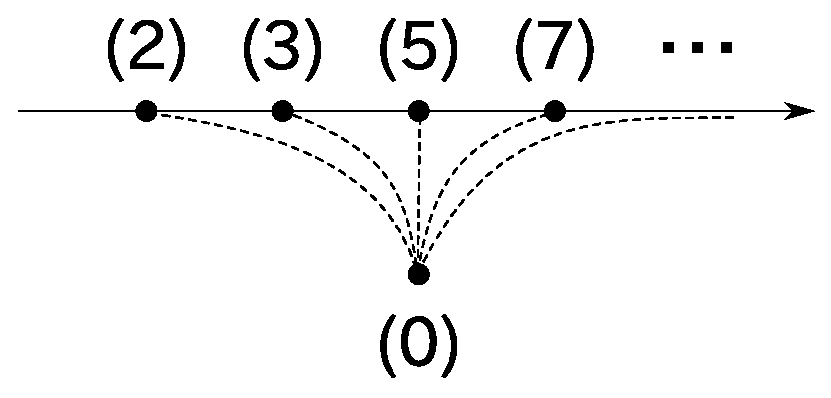
\includegraphics[width=5cm]{./images/SpecZ.eps}
    \end{center}
    \end{figure}

    任意の環$R$について,homomorphism $\phi: \Z \to R$を考える.
    準同型だから$\phi(0)=o, \phi(1)=e, \phi(-1)=-e$(ただし$o, e$はそれぞれ$R$の加法/乗法単位元.)となる.
    そして$\Z$は無限巡回群だから,$\phi(n-m)=\sum_{i=1}^n e+\sum_{i=1}^{m} (-e)$となり,
    よって準同型$\Z \to R$はただひとつ.
    つまり$|\Hom(\Z, R)|=1$.
    $\Spec \Z$はaffine spaceだから,Ex2.4より,任意のscheme $X$について$|\Hom(X, \Spec \Z)|=1$.
    すなわち,$\Spec \Z$は$\Sch$のfinal objectとなる.

\section{$\Spec \{0\}$ is the Initial Object in $\Sch$.} %% Ex2.6 
    零環$\{0\}$はただひとつのイデアル(したがって素イデアル)$(0)$を持つから,$\Spec \{0\}$は1点集合.
    零環から別の環への準同型写像は$0 \mapsto 0$なるものしか無い.
    schemeの間の射は環の間の準同型から作られるものしかないから(Prop2.3c),
    $\Spec \{0\}$から別のschemeへの射は$0 \mapsto 0$から得られるものしか無い.
    よって$\Spec \{0\}$はinitial object.

\section{Residue Field.} %% Ex2.7 
    Residue field of $x$ on $X$とは,剰余体$k(x):=\shO_{X,x}/\I{m}_{X,x}$のことである.

    $K$ :: field, $O:=(0) \subset K$とする.
    すると$\Spec K=\{O\}$であり,開集合は$\emptyset, \Spec K=\{O\}$の二つのみ.
    したがって$\shO_{\Spec K, O}=\shO_{\Spec K}(\Spec K)=K$となる.
    $\shO_{\Spec K, O}$は$\shO_{\Spec K}(\Spec K)$のみからなるdirect systemのdirect limitだから,
    これらは厳密に等しい.
    
    \paragraph{$(f,f^{\#}) \to (x, \phi)$}
    $(f, f^{\#}): (\Spec K, \shO_{\Spec K}) \to (X, \shO_X)$を考えよう.
    $f: \Spec K \to X$は,$\Spec K$が1点空間であることから,$f(O)$の値のみで定まる.
    この値を$x:=f(O)$としておこう.
    $f_* \shO_{\Spec K}$は
    \[
        f_* \shO_{\Spec K}(U)=
        \begin{cases}{}
            K & (x \in U) \\
            0 & (x \not \in U)
        \end{cases}
    \]
    で定まる.
    これは$K$のskyscraper sheaf (Ex.1.17)である.
    すると,$f^{\#}: \shO_X \to f_* \shO_{\Spec K}$は
    \[ (f^{\#})_{x}: \shO_{X,x} \to \shO_{\Spec K,f^{-1}(x)}=\shO_{\Spec K,O}=K \]
    を誘導する\footnote{$(f_* \shO)_P=\shO_{f^{-1}(P)}$を使った.}.
    これは以下の図式を可換にする射である.
    \[
    \xymatrix@C=5em
    {
    \shO_{X,x} \ar[r]^-{(f^{\#})_{x}} & \shO_{\Spec K,O} \\
    \shO_X(U) \ar[r]^-{(f^{\#})_U} \ar[u]_-{\mu_U} & \shO_{\Spec K}(\{O\}) \ar@{=}[u]
    }
    \]
    ただしこの図式では$x \in U \subseteq X$.
    $\im (f^{\#})_{x} \subseteq K$は体だから,第一同型定理より,$\ker (f^{\#})_{x}$は極大イデアル.
    よって$(f^{\#})_{x}$は
    \[ \xymatrix{ \shO_{X,x} \ar@{->>}[r]& \shO_{X,x}/\I{m}_{X,x}=k(x)~ \ar@{>->}[r]^-{\phi} & K } \]
    へと分解される.
    こうして$(f,f^{\#})$から$x \in X$と$\phi_f: k(x) \to K$が得られた.

    \paragraph{$(x, \phi) \to (f,f^{\#})$}
    逆に$x \in X$と$\phi: k(x) \to K$から$(f,f^{\#})$を作る.
    これには以上の手順を逆にたどればよい.
    まず$f$は以下のものになる.
    \begin{defmap}
        f:& \Spec K& \to& X \\ 
        {}& O& \mapsto& x
    \end{defmap}
    $\phi: k(x) \to K$から$f^{\#}$を復元するには,以下のようにする.
    \begin{defmap}
        f^{\#}_U:& \shO_X(U)& \to& (f_* \shO_{\Spec K})(U) \\ 
        {}& s& \mapsto&
        \begin{cases}{}
            \Phi_U(s) & (x \in U) \\
            0 & (x \not \in U)
        \end{cases}
    \end{defmap}
    ここでの$\Phi_U ~(\text{with }x \in U)$は,以下のような写像の結合である.
    \[
        \xymatrix
        {
            \shO_X(U) \ar[r]
            & \varinjlim_{x \in V} \shO_X(V)=\shO_{X,x} \ar@{->>}[r]
            & \shO_{X,x}/\I{m}_{X,x}=k(x) \ar[r]^-{\phi}
            & K=(f_* \shO_{\Spec K})(U)
        }
    \]
    $f^{\#}$から$\phi$を作った時,$\phi$から再び$f^{\#}$に戻ることは,
    前段落で見た二つの図式から分かる.

\section{ } %% Ex2.8 

\section{Uniquely-Existence of Generic Point.} %% Ex2.9 
    $X$をschemeとし,$Z$をそのnonempty irreducible closed subsetとする.
    この時,$Z$がただひとつのgeneric pointを持つことを示す.

    \paragraph{Useful Fact (!).}
    一般に,$D \subset X$が$X$のdense subsetならば,
    $X \setminus D$は空集合の他に開集合を含まない.
    これは直ちに理解できるが重要なので記しておく.

    \paragraph{Affine Case.}

    \paragraph{General Case.}
    affine open subset $U \subseteq X$であって,
    $U \cap Z \neq \emptyset$であるものをとる.
    この時,$U \cap Z$ ( :: closed in $U$)はaffine schemeのclosed subsetだから,
    前段落より,必ずgeneric point $\zeta$を持つ.
    この$\zeta$は$Z$のgeneric pointでもある.
    このことを示すために,$\{\zeta\}$が$Z$でdenseでないとしよう.
    すると$Z \setminus \{\zeta\}$は$V (\neq \emptyset)$ :: open in $Z$を含む.
    $Z$はirreducibleだから$V \cap U \neq \emptyset$.
    今$\zeta$は$Z \cap U$のgeneric pointとしたから,
    $(U \cap Z) \setminus \{\zeta\}=U \cap (Z \setminus \{\zeta\})$は
    $U \cap Z$の開集合を含まない.
    しかし今
    \[
        V \subseteq Z \setminus \{\zeta\}
        \text{ であり, }
        \emptyset \neq V \cap U \subseteq U \cap (Z \setminus \{\zeta\}).
    \]
    よって$\zeta \in U \cap Z$は$Z$のgeneric pointである.
    また,$\zeta$の他にgeneric point $\zeta'$が存在したとしよう.
    $\zeta' \not \in Z \cap U$であれば$Z \setminus \{\zeta'\}$は
    空でない開集合$Z \cap U$を含むことになるので,$\zeta, \zeta' \in Z \cap U$.
    前段落の結果より,$\zeta=\zeta'$が得られる.

%    $Z$の稠密部分集合全体$\Delta=\{D \subseteq Z \mid \overline{D}=Z \}$を考える.
%    $\Delta$は集合の包含関係についてpartially ordered setを成し,$Z \in \Delta$なので空ではない.
%    この時,$\delta=\bigcap \Delta=\bigcap_{D \in \Delta} D$とおく.
%    以下で$\delta$が稠密な1点集合であることを示す.
%    このことから$Z$がただひとつのgeneric pointを持つことがしたがう.

%    \paragraph{$\delta$ is Dense.}
%    $\delta$が稠密でないと仮定し,$\delta^c$を考える.
%    なので,仮定より,$\delta^c$は空でない開集合$U$を含む.
%    すると$\delta^c=\bigcup_{D \in \Delta} D^c$だから,
%    任意の$D \in \Delta$について$D^c \cap U$は$D^c$の開集合である.
%    さらに,少なくともひとつの$D_0 \in \Delta$について$D_0^c$は$U$と空でない交わりを持つ.
%    これは$D_0^c$が空でない開集合を含むということである.
%    $D_0$は稠密だから,これは矛盾.
%    (TODO: 示すべきは,$D_0^c$が空でない$Z$の開集合を含むということである.これでは$D_0^c$の相対位相での開集合の存在しか言えない.)

%    \paragraph{$\delta$ is One-Point Set.}
%    $\delta$が二点以上からなると仮定する.
%    この時,$\delta=\delta_1 \cup \delta_2$と,二つの異なる空でない部分集合にわけられる.
%    $\delta_1,\delta_2$は$\Delta$の極小元$\delta$よりも真に小さいから,以下が成り立つ.
%    \[
%        \bar{\delta_1}, \bar{\delta_2} \neq \emptyset, Z
%        \mand 
%        Z=\bar{\delta}=\overline{\delta_1 \cup \delta_2}=\bar{\delta_1} \cup \bar{\delta_2}=Z
%    \]
%    つまり,$Z$を二つの空でない真の閉集合の和として表せる.
%    しかし$Z$はirreducibleなのでこれはありえない.

\section{ } %% Ex2.10 

\section{ } %% Ex2.11 

\section{ } %% Ex2.12 

\section{ } %% Ex2.13 

\section{ } %% Ex2.14 

\section{ } %% Ex2.15 

\section{ } %% Ex2.16 

\section{ } %% Ex2.17 

\section{ } %% Ex2.18 

\section{ } %% Ex2.19 


\end{document}
